\section{Curvas y regiones en el plano complejo}
\label{sec:1_curvas_y_regiones_en_el_plano_complejo}

En esta sección se considerarán algunas curvas y regiones importantes, así como algunos conceptos relacionados con éstas, que serán usados con frecuencia. Lo anterior también será de ayuda para familiarizarse aún más con el plano complejo.

\subsection{Circunferencias y discos}

La distancia entre dos puntos $z$ y $a$ está dada por $\lvert z-a \rvert$. Por tanto, una circunferencia $C$ de radio $\rho$ y centro en $a$ puede definirse como
\begin{equation}
  \lvert z-a \rvert = \rho
  \label{eq:circ}
\end{equation}
Es decir, todos los puntos que equidistan de $a$ y su distancia es $\rho$. En la figura \ref{fig:circ_compx}, $z$ representa la circunferencia roja, es decir, todos los puntos que satisfacen \ref{eq:circ}
\begin{figure}[ht]
  \centering
  \begin{tikzpicture}[scale=0.7]
    \draw[->] (-1,0) -- (5,0) node[below right] {$\operatorname{Re}(z)$};
    \draw[->] (0,-1) -- (0,5) node[above left] {$\operatorname{Im}(z)$};
    \filldraw[blue] (2.5,2.5) circle (2pt) node[above right] {$a$};
    \draw[red] (2.5,2.5) circle (1.5);
    \draw[teal] (2.5,2.5) -- (1,2.5) node[midway, above] {$\color{teal}\rho$};
  \end{tikzpicture}
  \caption{Circunferencia en el plano complejo.}
  \label{fig:circ_compx}
\end{figure}

En particular, la circunferencia unitaria; es decir, la circunferencia de radio 1 y centro en el origen $a=0$, es
\begin{equation*}
  \lvert z \rvert = 1
\end{equation*}

Además, la desigualdad
\begin{equation}
  \lvert z - a \rvert < \rho
  \label{eq:inter_circ}
\end{equation}
se cumple para todo punto $z$ dentro de $C$; es decir, \ref{eq:inter_circ} representa el interior de $C$, esta región se denomina disco circular o, más precisamente, disco \textit{abierto}, en contraste con el disco circular \textit{cerrado}.
\begin{equation*}
  \lvert z-a \rvert \leqslant \rho
\end{equation*}
el cual consta del interior de $C$ y la propia $C$. El disco circular abierto \ref{eq:inter_circ} se denomina también \textbf{vecindad} del punto $a$. Resulta evidente que $a$ tiene una infinidad de tales vecindades, cada una de las cuales corresponde a un cierto valor de $\rho$ (>0), y $a$ es un punto de cada una de tales vecindades.
\label{word:vecindad}

De manera semejante, la desigualdad 
\begin{equation*}
  \lvert z-a \rvert > \rho
\end{equation*}
representa el exterior del círculo $C$. Además, la región entre dos círculos concétricos de radios $\rho_1$ y $\rho_2$ (>$\rho_1$) puede definirse como
\begin{equation}
  \rho_1 < \lvert z-a \rvert < \rho_2,
\end{equation}
en donde $a$ es el centro de los círculos. Tal región se denomina \textit{anillo circular abierto} o \textbf{corona} abierta (figura \ref{fig:corona_complx}).
\begin{figure}[ht]
  \centering
  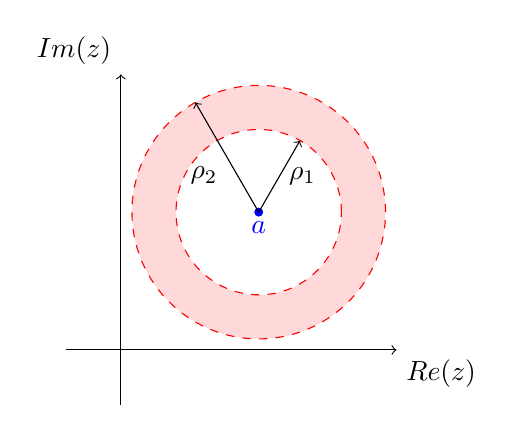
\begin{tikzpicture}[scale=0.7]
    % Ejes
    \draw[->] (-1,0) -- (5,0) node[below right] {$\operatorname{Re}(z)$};
    \draw[->] (0,-1) -- (0,5) node[above left] {$\operatorname{Im}(z)$};

    % Centro a
    \filldraw[blue] (2.5,2.5) circle (2pt) node[below] {$a$};

    % Región sombreada entre las dos circunferencias
    \fill[red!15, even odd rule] 
      (2.5,2.5) circle (2.3)
      (2.5,2.5) circle (1.5);

    % Contornos
    \draw[red, dashed] (2.5,2.5) circle (1.5);
    \draw[red, dashed] (2.5,2.5) circle (2.3);

    % Radio de la menor
    \draw[->] (2.5,2.5) -- ++(60:1.5)
      node[midway, right] {$\rho_1$};
    % Radio de la mayor
    \draw[->] (2.5,2.5) -- ++(120:2.3)
      node[midway, below left] {$\rho_2$};
  \end{tikzpicture}
  \caption{Corona en el plano complejo.}
  \label{fig:corona_complx}
\end{figure}

Veamos un ejemplo.
\begin{example}
  Determinar la región en el plano complejo definida por $\lvert z-3+j\rvert\leqslant4$.

  \textbf{Solución}: La desigualdad es válida precisamente para todos los $z$ cuya distancia a $a=3-j$ no es mayor que $4$. Por tanto, se trata de un disco circular cerrado de radio $4$ con centro en $3-j$.

  Gráficamente tenemos
  \begin{figure}[ht]
    \centering
    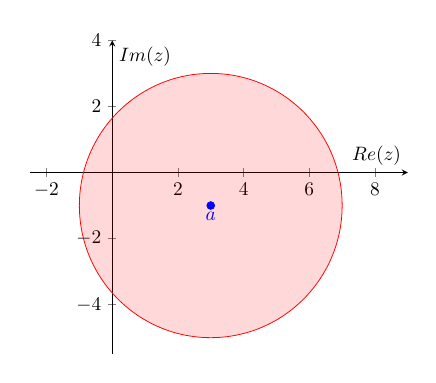
\begin{tikzpicture}[scale=0.7]
      \begin{axis}[
        axis lines = middle,
        xlabel = {$\operatorname{Re}(z)$},
        ylabel = {$\operatorname{Im}(z)$},
        xmin=-2.5, xmax=9,
        ymin=-5.5, ymax=4,
        ]
        \draw[red] (3,-1) circle (4);
        \fill[red, opacity=0.15] (3,-1) circle (4);
        \filldraw[blue] (3,-1) circle (2pt) node[below] {$a$};
      \end{axis}
    \end{tikzpicture}
  \end{figure}
\end{example}

\subsection{Semiplanos}

Por semiplano superior (abierto) se entiende el conjunto de todos los puntos $z=x+jy$ tales que $y>0$. De manera semejante, la condición $y<0$ define el semiplano inferior, $x>0$ el semiplano derecho y $x<0$ el semiplano izquierdo.

\subsection{Conceptos de conjuntos en el plano complejo}

Por último, a continuación se enumeran brevemente algunos conceptos de interés general que serán usados posteriormente; aquí se plantean para referencias según sean necesarios.

El término \textbf{conjunto de puntos} en el plano complejo significa cualquier colección finita o infinita de tales puntos. Por ejemplo, las soluciones de una ecuación cuadrática, los puntos de una recta y los puntos en el interior de un circulo son conjuntos de puntos.

Un conjunto $S$ se denomina \textbf{abierto} si cualquier punto de $S$ tiene una vecindad (definido en \ref{word:vecindad}) que consta completamente de puntos que pertenecen a $S$. Matemáticamente hablando, el conjunto $S \subset \mathbb{C}$ es abierto si para todo punto $a \in S$ existe un número $\rho > 0$ tal que toda la vecindad
\[
V(a,\rho) = \{z \in \mathbb{C} : |z - a| < \rho\}
\]
está completamente contenida en \( S \).

Dicho más gráficamente: si te colocas sobre cualquier punto de \( S \), puedes dibujar un pequeño círculo alrededor tuyo que no se salga de \( S \). Veamos un ejemplo.
\begin{example}\label{ej:conjunto_cerrado}
  Supongamos un conjunto de puntos $\lvert z-a\rvert \leqslant r$
  \[
  S = \{z \in \mathbb{C} : |z - a| \leqslant r\}.
  \]
  Este es el disco cerrado de radio \(r\) centrado en \(a\). Incluye todos los puntos dentro del círculo y también los puntos del borde donde \(|z - a| = r\).

  La pregunta es: ¿cumple la definición de conjunto abierto? Analicemos:
  \begin{itemize}
  \item Toma un punto \(z_0\) en el interior, es decir con \(|z_0 - a| < r\).
   Aquí sí puedes encontrar un \(\rho > 0\) tal que todo \(z\) con \(|z - z_0| < \rho\) también satisfaga \(|z - a| < r\).
   Es decir, los puntos interiores cumplen la condición.

  \item Toma ahora un punto \(z_0\) en el borde, con \(|z_0 - a| = r\).
    No importa cuán pequeño elijas \(\rho > 0\), siempre habrá puntos dentro del círculo \(|z - z_0| < \rho\) que estén fuera del disco, es decir que satisfagan \(|z - a| > r\).
    Por tanto, ninguna vecindad de \(z_0\) está completamente contenida en \(S\).
  \end{itemize}
  Así que el conjunto falla la condición para los puntos del borde.

  Conclusión:
  \[
  \boxed{{z : |z - a| \leqslant r} \text{ no es abierto.}}
  \]
  Es un conjunto cerrado, porque contiene a todos sus puntos frontera. En cambio,
  \[
  {z : |z - a| < r}
  \]
  sí es abierto, porque todo punto dentro tiene una vecindad contenida en el conjunto.
\end{example}

Se dice que un conjunto abierto $S$ es \textbf{conexo} si dos puntos cualesquiera de $S$ pueden unirse mediante una línea quebrada constituida por un número finito de segmentos de recta completamente contenidos en $S$. Un conjunto conexo abierto se denomina \textbf{dominio}. Así un disco abierto o una corona abierta (como la figura \ref{fig:corona_complx}) son dominios. Un cuadrado abierto sin una diagonal no es un dominio (¿por qué?). Como se ve en la figura \ref{fig:cuadrado_abierto}, podemos colocar dos puntos tales que el la línea quebrada deba cortar la diagonal faltante. Esto significa que el conjunto no es conexo.
\begin{figure}[ht]
  \centering
  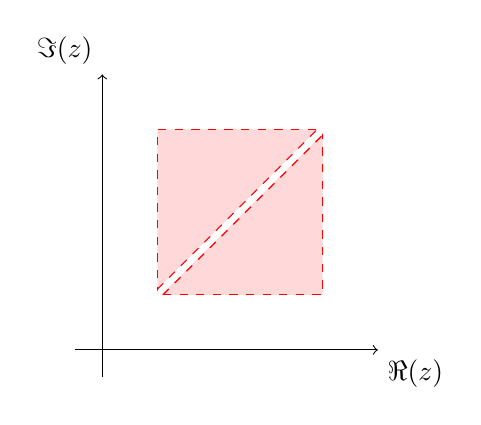
\begin{tikzpicture}[scale=0.7]
    \draw[->] (-0.5,0) -- (5,0) node[below right] {$\Re(z)$};
    \draw[->] (0,-0.5) -- (0,5) node[above left] {$\Im(z)$};

    \fill[red!15, even odd rule]
          (1,1) rectangle (4,4)  % exterior: el cuadrado
          (1,1) -- (4,4) -- (3.9,4) -- (1,1.1) -- cycle;
    \draw[dashed, red] (1,1) rectangle (4,4);
    \draw[white, line width=2pt] (1,1) -- (4,4); % “borra” una línea ancha

    \draw[red, dashed] (1.1,1) -- (4,3.9);
    \draw[red, dashed] (1,1.1) -- (3.9,4);
  \end{tikzpicture}
  \caption{Región cuadrada abierta sin una diagonal}
  \label{fig:cuadrado_abierto}
\end{figure}

El \textbf{complemento} de un conjunto $S$ en el plano complejo es el conjunto de todos los puntos del plano complejo que \textit{no} pertenecen a $S$. Un conjunto $S$ se denomina cerrado si su complemento es abierto. Por ejemplo, los puntos sobre y en el interior del círculo unitario constituyen un conjunto cerrado (``disco unitario cerrado''), ya que su complemento $\lvert z \rvert > 1$ es abierto.

Un \textbf{punto frontera} de un conjunto $S$ es aquel para el que toda vecindad contiene puntos que pertenecen a $S$ y puntos que \textit{no} pertenecen a $S$. En el ejemplo \ref{ej:conjunto_cerrado} vimos que los puntos del borde de la circunferencia son puntos frontera, ya que la vecindad de cada punto incluye puntos que pertenecen a $S$ y puntos que no pertenecen a $S$.

Una \textbf{región} es un conjunto que consta de un dominio más, quizá, algunos o todos sus puntos frontera. 
